\documentclass[10pt]{article} 

\setlength{\oddsidemargin}{0.0in}
\setlength{\evensidemargin}{0.0in}
\setlength{\topmargin}{-0.25in}
\setlength{\headheight}{0in}
\setlength{\headsep}{0in}
\setlength{\textwidth}{6.5in}
\setlength{\textheight}{9.25in}
\setlength{\parindent}{0in}
\setlength{\parskip}{2mm}

\usepackage{graphicx}
\DeclareGraphicsExtensions{.png}

\begin{document}

\title{\textbf{ECS 171 Homework 2 Report}}
\author{Parker Temple, 997223534, Section 1}
\maketitle

\begin{flushleft}

\section{3 layer ANN. Data Split into random 75\% training set, 25\% testing set.}

Testing Error: 0.522911

Error change over all batches

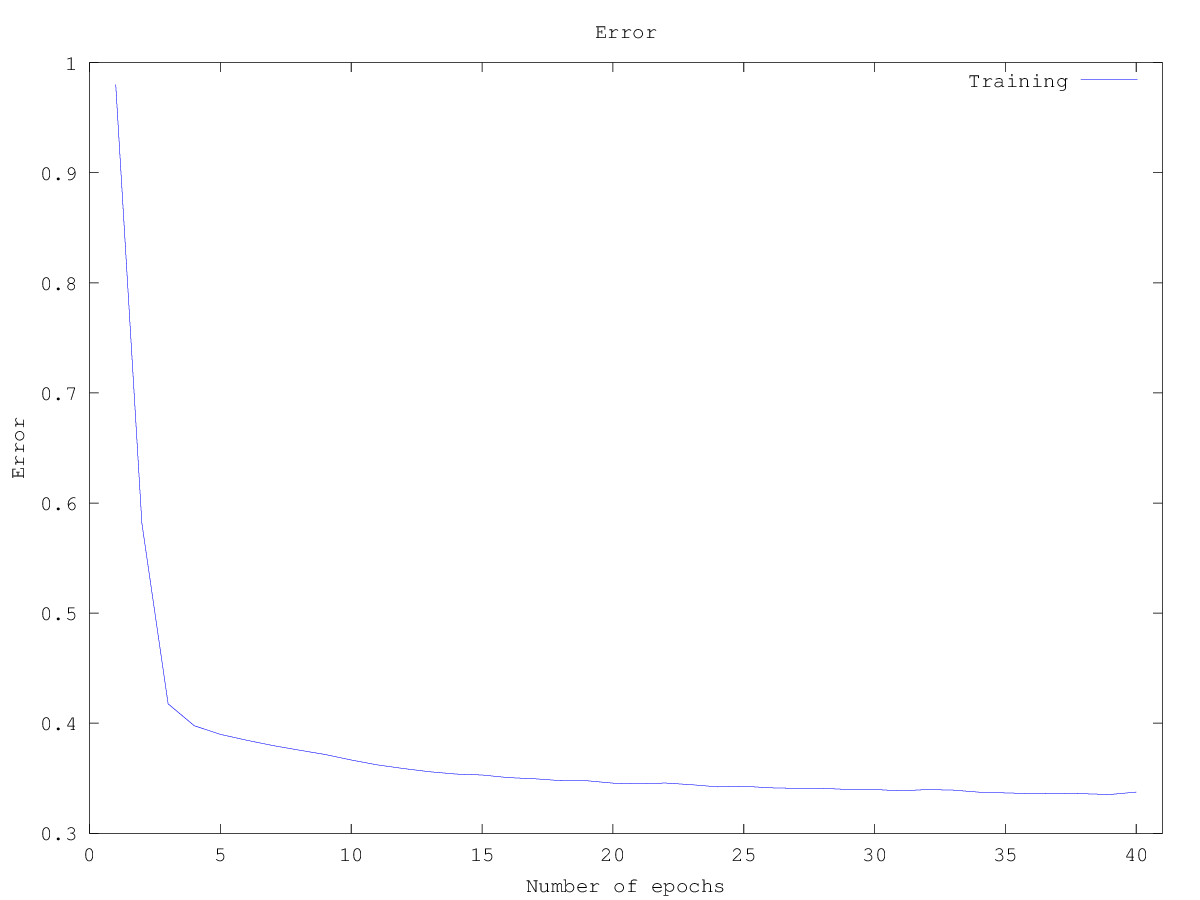
\includegraphics[width=\linewidth]{./errorplot.png}

\newpage

Change of 67 weights for first 50 iterations. 8 weights per graph, the bottom right graph, which has 11 weights on it.

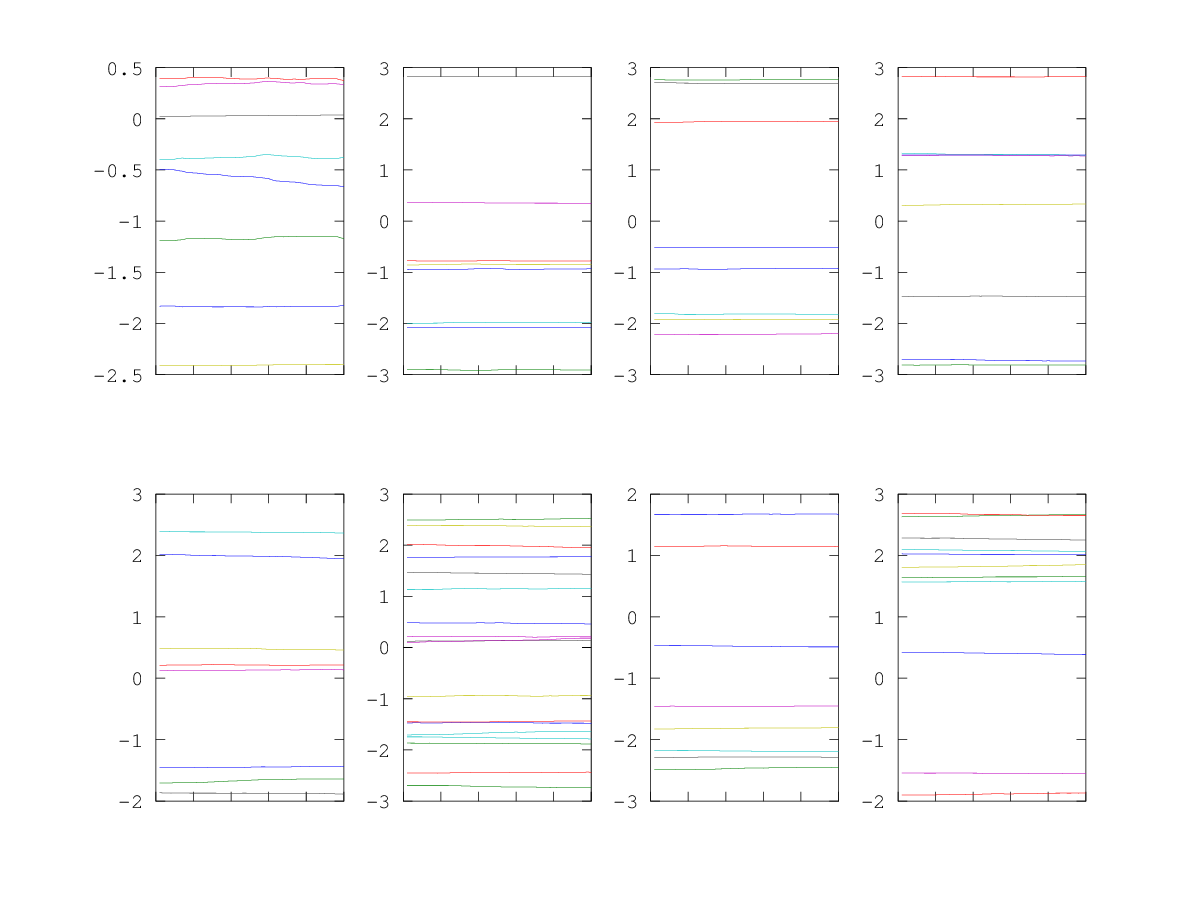
\includegraphics[width=\linewidth]{./weightchange.png}

\newpage

Change of the 10 output activations for first 50 iterations. 1 activation per graph.

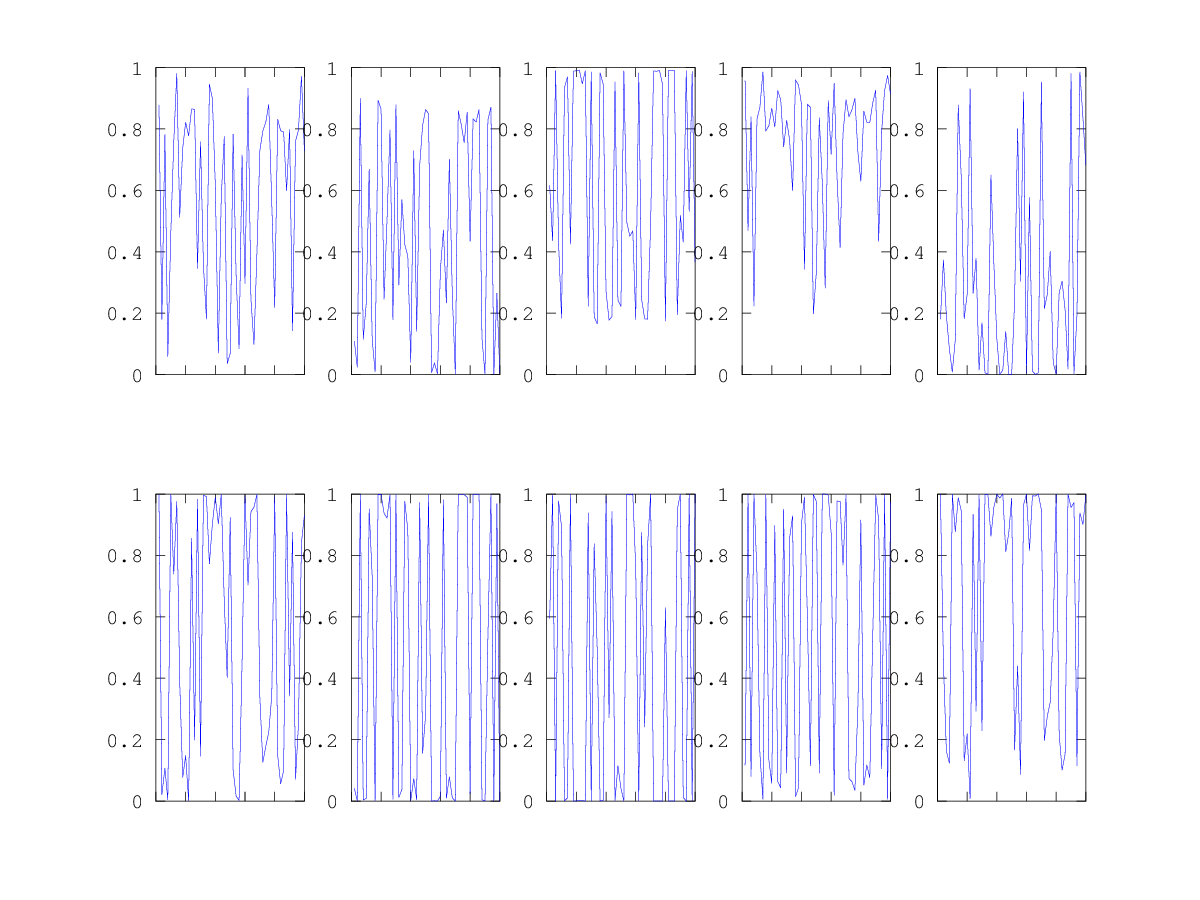
\includegraphics[width=\linewidth]{./outputchange.png}

\section{Training error, $\alpha_i$ equations}
Training Error: 0.449461

Activation function equations

\tiny
$a_{1}^{(2)} = g(2.164202 \cdot x_{0}+0.176168 \cdot x_{1}+0.213492 \cdot x_{2}+1.503652 \cdot x_{3}+0.215892 \cdot x_{4}+-1.486713 \cdot x_{5}+1.820079 \cdot x_{6}+-0.042223 \cdot x_{7}+0.035219 \cdot x_{8})$
$a_{2}^{(2)} = g(0.543049 \cdot x_{0}+0.230263 \cdot x_{1}+0.790381 \cdot x_{2}+-0.202021 \cdot x_{3}+1.330253 \cdot x_{4}+2.516649 \cdot x_{5}+2.473374 \cdot x_{6}+0.390521 \cdot x_{7}+-2.431607 \cdot x_{8})$
$a_{3}^{(2)} = g(-2.162728 \cdot x_{0}+-0.260760 \cdot x_{1}+0.081877 \cdot x_{2}+-0.012670 \cdot x_{3}+0.361112 \cdot x_{4}+3.017692 \cdot x_{5}+-0.953964 \cdot x_{6}+0.203506 \cdot x_{7}+-0.100807 \cdot x_{8})$

\scriptsize
$a_{1}^{(3)} = g(-0.905029 \cdot x_{0}+0.878869 \cdot a_{1}^{(2)}+-0.109502 \cdot a_{2}^{(2)}+0.665166 \cdot a_{3}^{(2)})$
$a_{2}^{(3)} = g(0.370766 \cdot x_{0}+1.329797 \cdot a_{1}^{(2)}+-0.954598 \cdot a_{2}^{(2)}+2.167791 \cdot a_{3}^{(2)})$
$a_{3}^{(3)} = g(0.983497 \cdot x_{0}+0.774112 \cdot a_{1}^{(2)}+1.339974 \cdot a_{2}^{(2)}+3.257448 \cdot a_{3}^{(2)})$
$a_{4}^{(3)} = g(0.785000 \cdot x_{0}+-2.476845 \cdot a_{1}^{(2)}+0.237973 \cdot a_{2}^{(2)}+0.008546 \cdot a_{3}^{(2)})$
$a_{5}^{(3)} = g(0.120132 \cdot x_{0}+-1.080554 \cdot a_{1}^{(2)}+-0.227997 \cdot a_{2}^{(2)}+2.504238 \cdot a_{3}^{(2)})$
$a_{6}^{(3)} = g(-2.905498 \cdot x_{0}+1.017531 \cdot a_{1}^{(2)}+-1.459890 \cdot a_{2}^{(2)}+3.087088 \cdot a_{3}^{(2)})$
$a_{7}^{(3)} = g(0.169951 \cdot x_{0}+-1.243626 \cdot a_{1}^{(2)}+-0.254528 \cdot a_{2}^{(2)}+2.601597 \cdot a_{3}^{(2)})$
$a_{8}^{(3)} = g(-2.129364 \cdot x_{0}+-0.451775 \cdot a_{1}^{(2)}+-0.510962 \cdot a_{2}^{(2)}+0.661315 \cdot a_{3}^{(2)})$
$a_{9}^{(3)} = g(-3.955992 \cdot x_{0}+0.606784 \cdot a_{1}^{(2)}+0.561681 \cdot a_{2}^{(2)}+0.857540 \cdot a_{3}^{(2)})$
$a_{10}^{(3)} = g(-0.370148 \cdot x_{0}+-1.814781 \cdot a_{1}^{(2)}+-0.578687 \cdot a_{2}^{(2)}+2.764005 \cdot a_{3}^{(2)})$


\normalsize
\newpage

\section{Hand calculations}

\small

First sample: 

X Values

   0.91254   1.04527   0.42585  -1.07846   0.55858  -1.65363   0.47010  -0.68026

Y Value

   0   0   1   0   0   0   0   0   0   0

Initial weights

{

  [1,1] =

     1   1   1   1   1   1   1   1   1

     1   1   1   1   1   1   1   1   1

     1   1   1   1   1   1   1   1   1

  [1,2] =

     1   1   1   1

     1   1   1   1

     1   1   1   1

     1   1   1   1

     1   1   1   1

     1   1   1   1

     1   1   1   1

     1   1   1   1

     1   1   1   1

     1   1   1   1

}

Updated weights

{
  [1,1] =

     0.99882   0.99893   0.99877   0.99950   1.00127   0.99934   1.00195   0.99945   1.00080

     0.99882   0.99893   0.99877   0.99950   1.00127   0.99934   1.00195   0.99945   1.00080

     0.99882   0.99893   0.99877   0.99950   1.00127   0.99934   1.00195   0.99945   1.00080

  [1,2] =

     0.99983   0.99983   0.99983   0.99983

     0.99983   0.99983   0.99983   0.99983

     1.00000   1.00000   1.00000   1.00000

     0.99983   0.99983   0.99983   0.99983

     0.99983   0.99983   0.99983   0.99983

     0.99983   0.99983   0.99983   0.99983

     0.99983   0.99983   0.99983   0.99983

     0.99983   0.99983   0.99983   0.99983

     0.99983   0.99983   0.99983   0.99983

     0.99983   0.99983   0.99983   0.99983

}

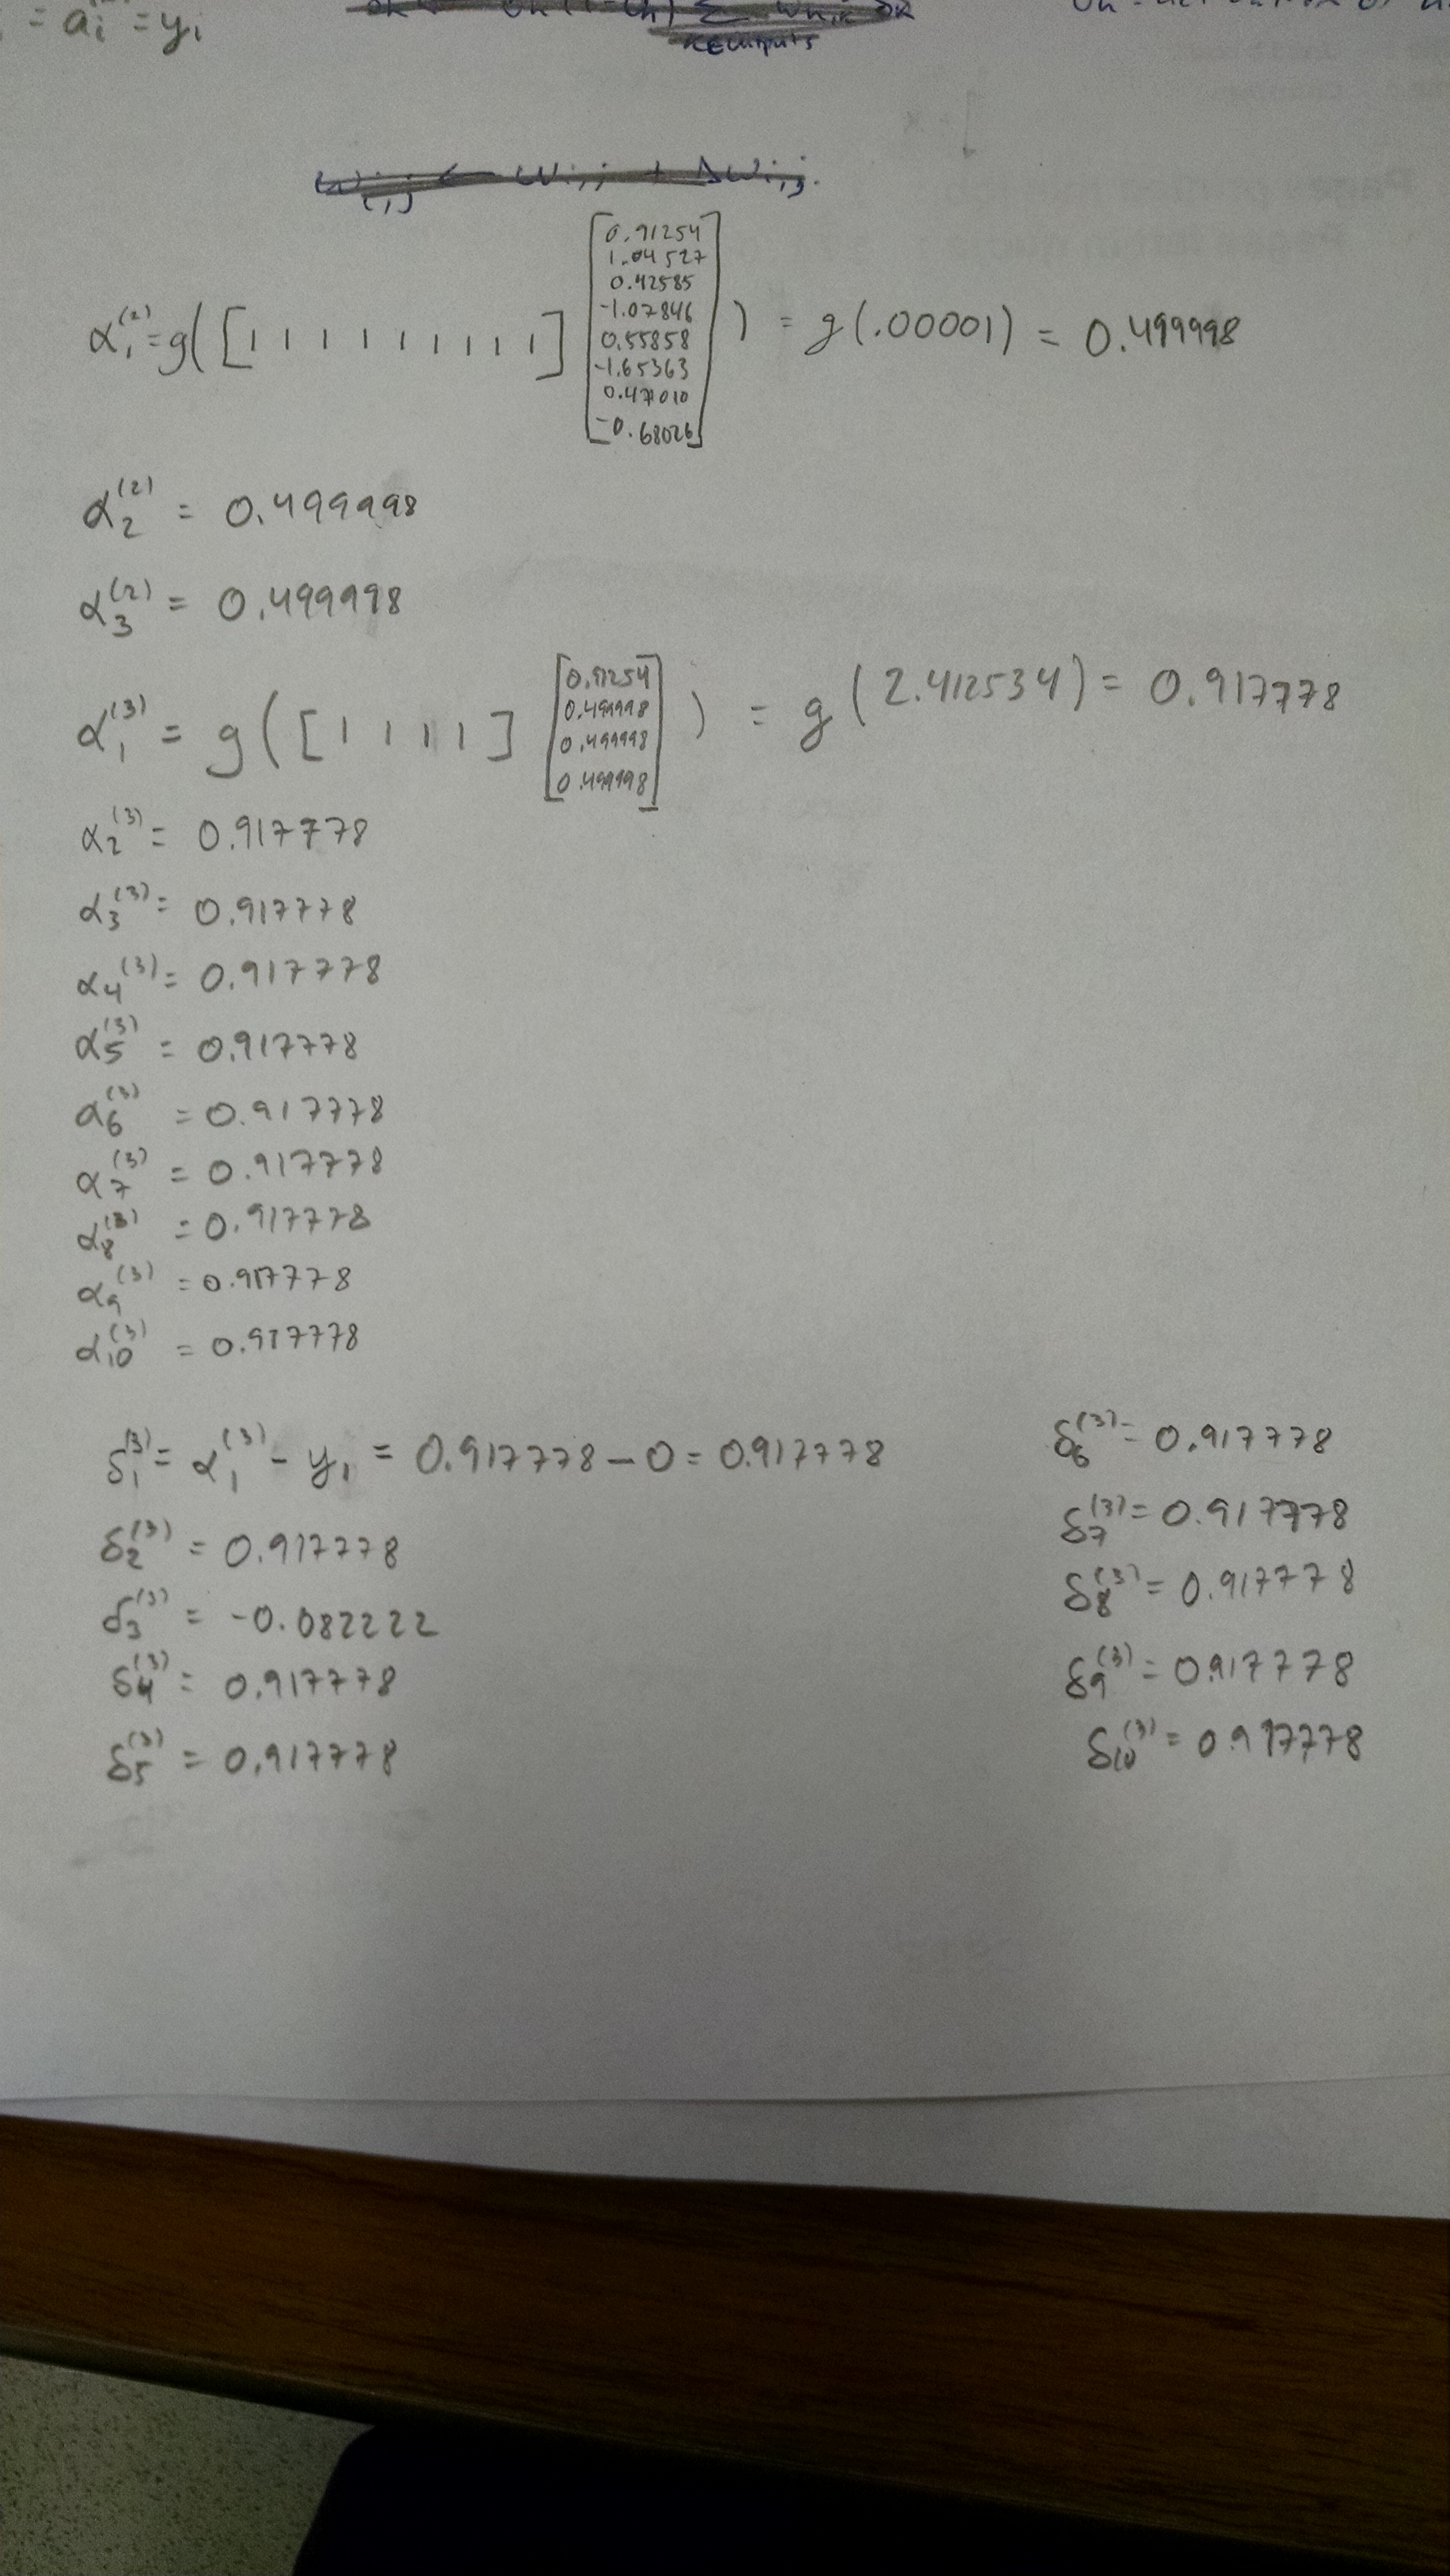
\includegraphics[width=\linewidth,height=\textheight]{./hand1.jpg}

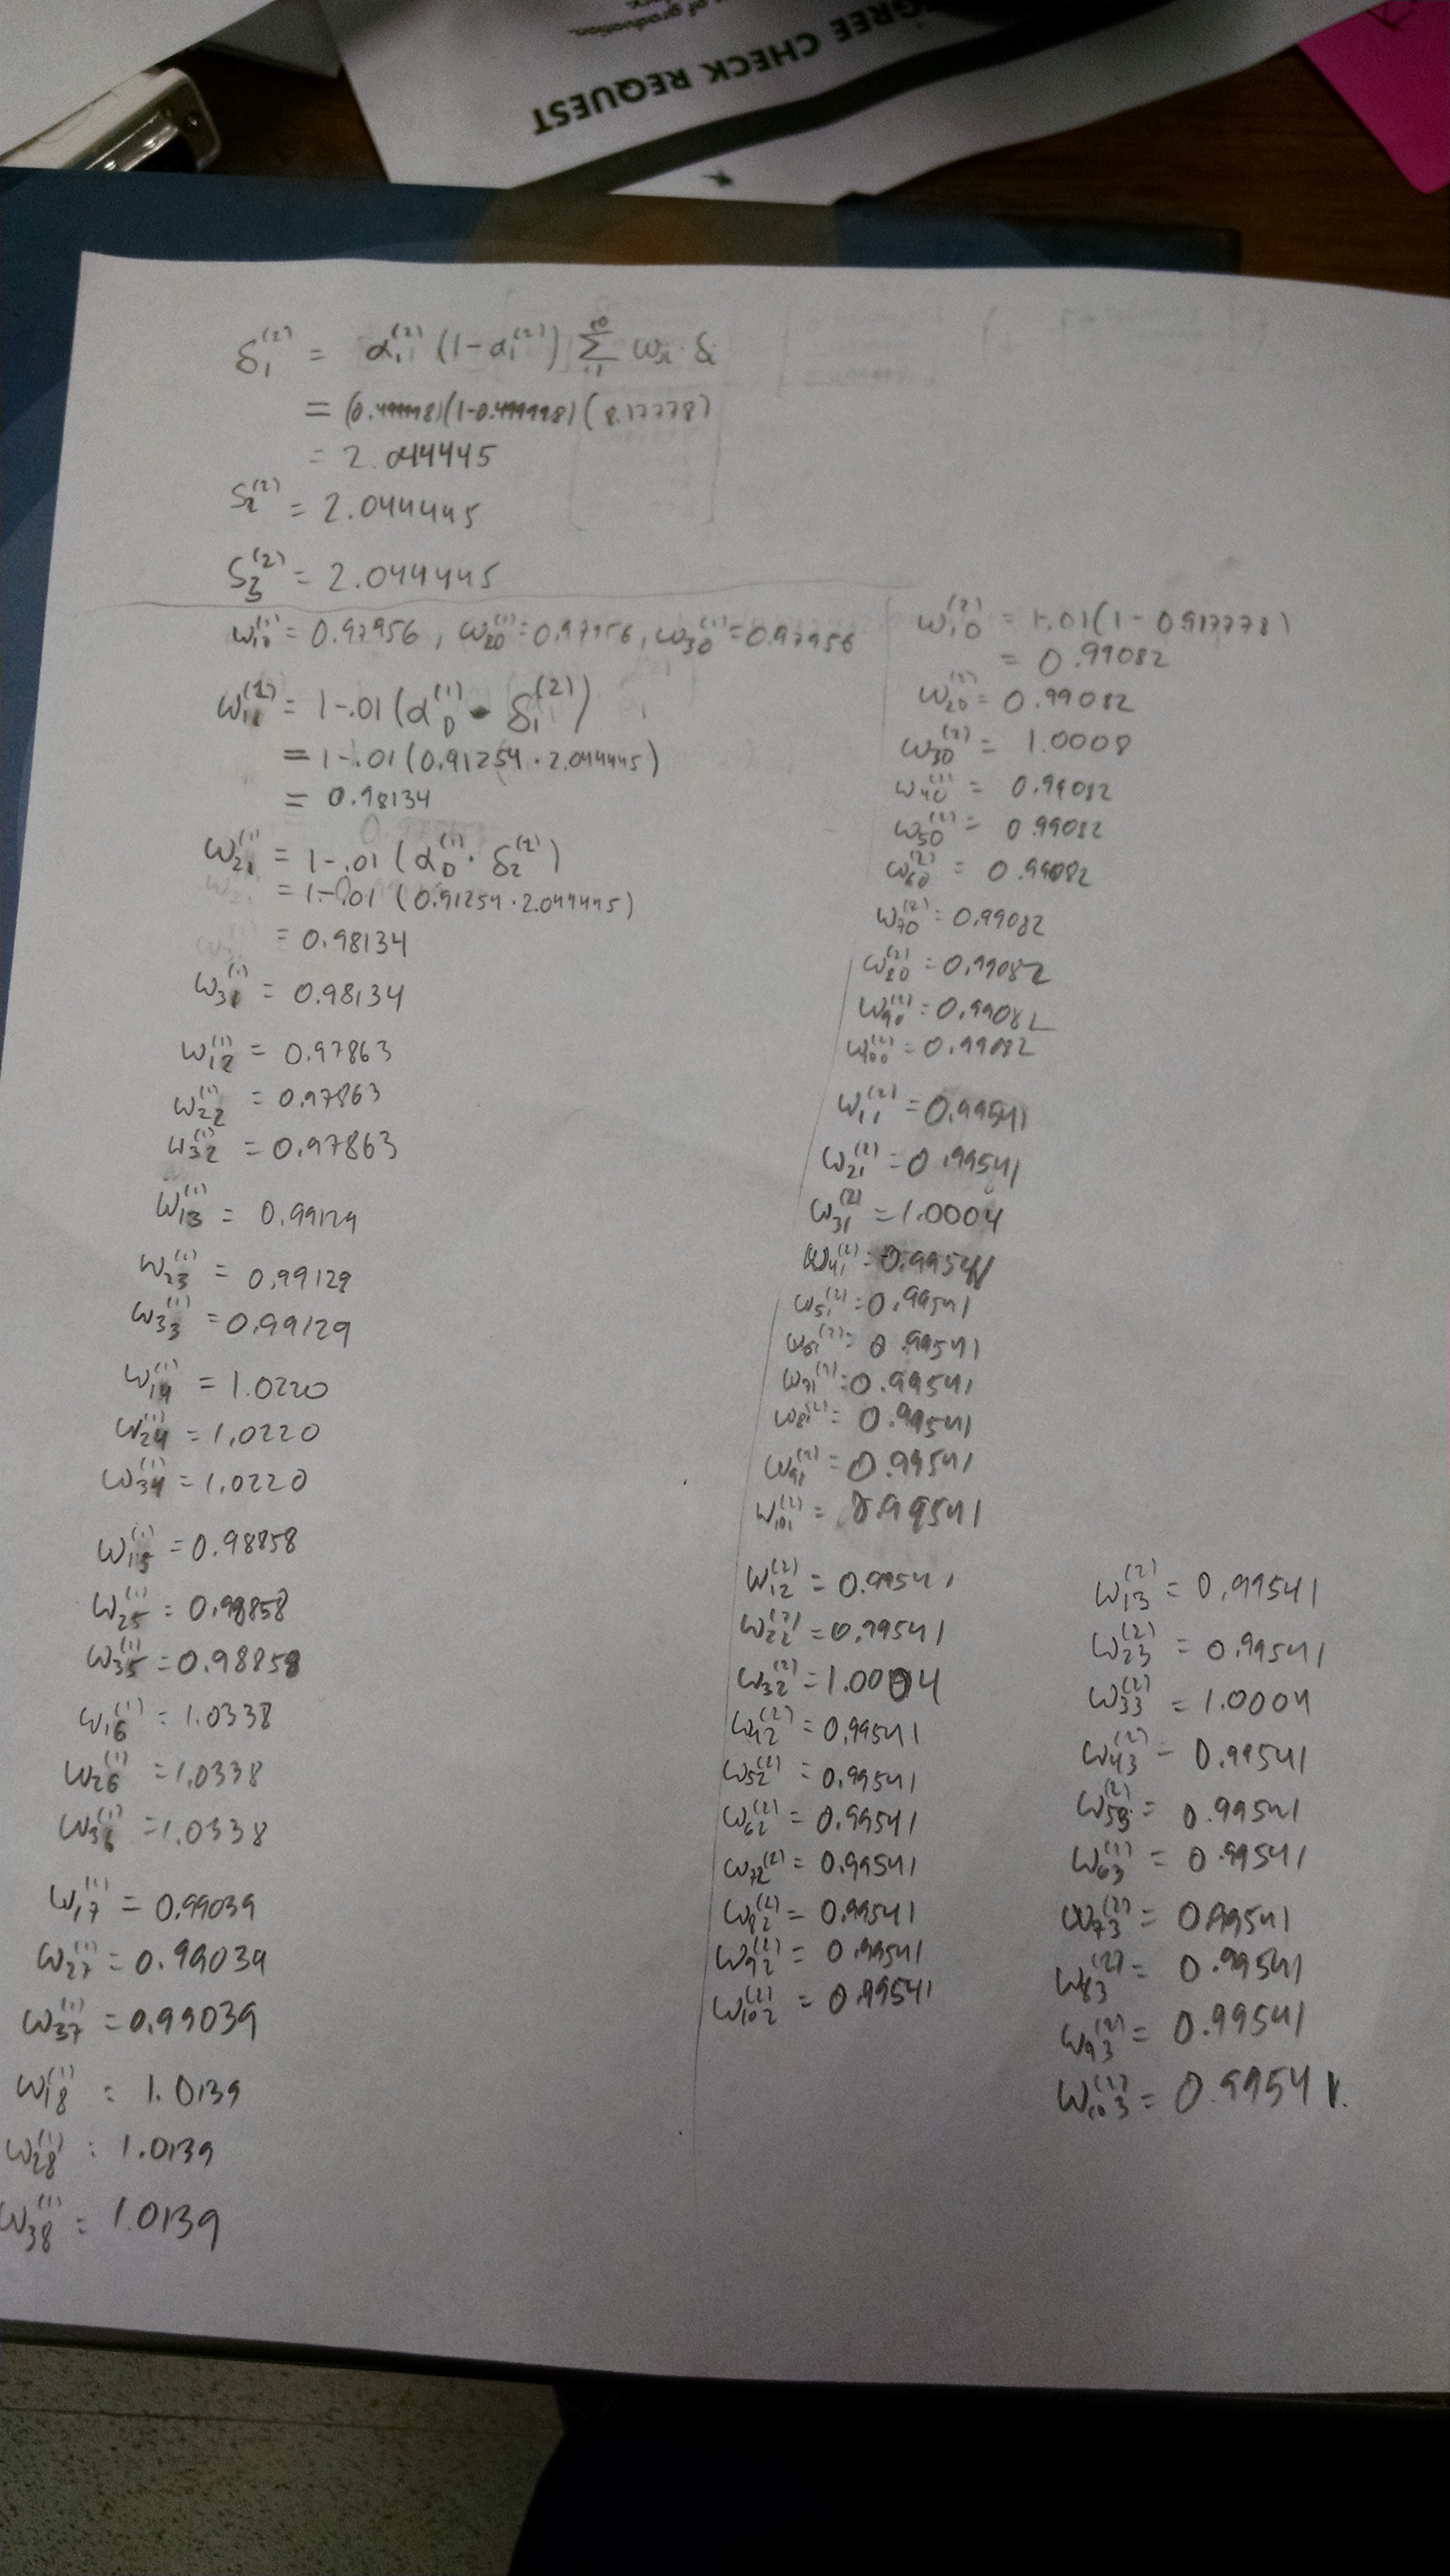
\includegraphics[width=\linewidth,height=\textheight]{./hand2.jpg}

\normalsize

\newpage

\section{Change number of hidden layers and number of nodes per hidden layer}

3 by 4 matrix of testing errors. Rows are 1 layer, 2 layers, 3 layers. Columns are 3 nodes per layer, 5 nodes, 8 nodes, 10 nodes.

   0.54313   0.40970   0.41712   0.38544

   0.50943   0.44609   0.42385   0.38544

   0.62601   0.47978   0.51011   0.37736

The optimal configuration is 3 hidden layers with 10 nodes per layer.

The relationship between these attributes and the generalization error is that as nodes per hidden layer increase, error decreases, but as the number of hidden layers increases, the error tends to increase. This is probably due to the fact that more layers substantially increases intra-neuron interactions, and is similar to creating a higher order polynomial. This can lead to overfitting. 

\section{Sample prediction}

Unknown sample prediction: MIT

\section{Uncertainty Measures}

If we average all the other percent likelihoods of the output nodes excluding the one that was the maximum, we can get an average percent uncertainty. The percent uncertainty of the unknown sample is 0.12315. This a simiplisitic model for predicting uncertainty.

\end{flushleft}
\end{document} 
